% Format teze zasnovan je na paketu memoir
% http://tug.ctan.org/macros/latex/contrib/memoir/memman.pdf ili
% http://texdoc.net/texmf-dist/doc/latex/memoir/memman.pdf
% 
% Prilikom zadavanja klase memoir, navedenim opcijama se podešava 
% veličina slova (12pt) i jednostrano štampanje (oneside).
% Ove parametre možete menjati samo ako pravite nezvanične verzije
% mastera za privatnu upotrebu (na primer, u b5 varijanti ima smisla 
% smanjiti 
\documentclass[12pt,oneside]{memoir} 

% Paket koji definiše sve specifičnosti master rada Matematičkog fakulteta
\usepackage[latinica]{matfmaster} 
\usepackage{elm-highlighting}

\usepackage{listings,xcolor}
    \usepackage[T1]{fontenc}
    \usepackage{xcolor}
    \usepackage[scaled=0.9]{DejaVuSansMono}
\definecolor{commentgreen}{RGB}{2,112,10}
\definecolor{eminence}{RGB}{108,48,130}
\definecolor{weborange}{RGB}{255,165,0}
\definecolor{frenchplum}{RGB}{129,20,83}

\lstdefinelanguage{elixir}{
    morekeywords={case,catch,def,do,else,false,%
        use,alias,receive,timeout,defmacro,defp,%
        for,if,import,defmodule,defprotocol,%
        nil,defmacrop,defoverridable,defimpl,%
        super,fn,raise,true,try,end,with,%
        unless},
    otherkeywords={<-,->, |>, \%\{, \}, \{, \, (, )},
    sensitive=true,
    morecomment=[l]{\#},
    morecomment=[n]{/*}{*/},
    morecomment=[s][\color{purple}]{:}{\ },
    morestring=[s][\color{orange}]"",
    commentstyle=\color{commentgreen},
    keywordstyle=\color{eminence},
    stringstyle=\color{red},
	basicstyle=\ttfamily,
	breaklines,
	showstringspaces=false,
	frame=tb
}


%

%

%
% Opcija [biblatex]:
%   ako želite da koristite reference na više jezika i umesto paketa
%   bibtex da koristite BibLaTeX/Biber, dodajte opciju "biblatex" tj.
%   prethodni paket uključite pomoću: \usepackage[biblatex]{matfmaster}
%
% Opcija [b5paper]:
%   ako želite da napravite verziju teze u manjem (b5) formatu, navedite
%   opciju "b5paper", tj. prethodni paket uključite pomoću: 
%   \usepackage[b5paper]{matfmaster}. Tada ima smisla razmisliti o promeni
%   veličine slova (izmenom opcije 12pt na 11pt u \documentclass{memoir}).
%
% Naravno, opcije je moguće kombinovati.
% Npr. \usepackage[b5paper,biblatex]{matfmaster}


% Datoteka sa literaturom u BibTex tj. BibLaTeX/Biber formatu
\bib{matfmaster-primer}

% Ime kandidata na srpskom jeziku (u odabranom pismu)
\autor{Ana Petrović}
% Naslov teze na srpskom jeziku (u odabranom pismu)
\naslov{Testiranje funkcionalnog koda}
% Godina u kojoj je teza predana komisiji
\godina{2023}
% Ime i afilijacija mentora (u odabranom pismu)
\mentor{dr Ime\textsc{Prezime}, redovan profesor\\ Univerzitet u Beogradu, Matematički fakultet}
% Ime i afilijacija prvog člana komisije (u odabranom pismu)
\komisijaA{dr Ime \textsc{Prezime}, vanredni profesor\\ University of Disneyland, Nedođija}
% Ime i afilijacija drugog člana komisije (u odabranom pismu)
\komisijaB{dr Ime \textsc{Prezime}, docent\\ Univerzitet u Beogradu, Matematički fakultet}
% Ime i afilijacija trećeg člana komisije (opciono)
% \komisijaC{}
% Ime i afilijacija četvrtog člana komisije (opciono)
% \komisijaD{}
% Datum odbrane (odkomentarisati narednu liniju i upisati datum odbrane ako je poznat)
% \datumodbrane{}

% Apstrakt na srpskom jeziku (u odabranom pismu)
\apstr{%
Apstrakt
}

% Ključne reči na srpskom jeziku (u odabranom pismu)
\kljucnereci{funkcionalno programiranje, testiranje, verifikacija softvera, programski jezik Elixir, programski jezik Elm}

\begin{document}
% ==============================================================================
% Uvodni deo teze
\frontmatter
% ==============================================================================
% Naslovna strana
\naslovna
% Strana sa podacima o mentoru i članovima komisije
\komisija
% Strana sa posvetom (u odabranom pismu)
%\posveta{Mami, tati i dedi}
% Strana sa podacima o disertaciji na srpskom jeziku
\apstrakt
% Sadržaj teze
\tableofcontents*

% ==============================================================================
% Glavni deo teze
\mainmatter
% ==============================================================================

% ------------------------------------------------------------------------------
\chapter{Uvod}
% ------------------------------------------------------------------------------

Ovde ide uvod .. ... ..... 

% ------------------------------------------------------------------------------
\chapter{Funkcionalna paradigma}
\label{chp:uvodnideo}

\par Funkcionalno programiranje je specifičan pristup programiranju, tj. programska paradigma, koja se zasniva na pojmu matematičke funkcije. Programi se kreiraju pomoću izraza i funkcija, bez izmena stanja i podataka \cite{func}. Iz tog razloga, jednostavniji su za razumevanje i otporniji na greške u odnosu na imperativne programe. U slučaju funkcionalnih programskih jezika, osnovna apstrakcija je \textit{funkcija}. Programski stil je deklarativnog tipa i umesto naredbi koriste se izrazi, tako da se izvršavanje programa svodi na evaluaciju izraza. Vrednost izraza je nezavisna od konteksta u kojem se izraz nalazi. Osnovna osobina čistih funkcionalnih jezika (eng. \textit{pure functional programming language}) jeste transparentnost referenci, što kao posledicu ima nepostojanje propratnih efekata. Sa druge strane, nečisti funkcionalni jezici (eng. \textit{impure functional programming language}) su manje elegantni jer dozvoljavaju bočne efekte, koji mogu izazvati suptilne greške i biti teži za razumevanje. Međutim, praktičniji su za specifične vrste zadataka, kao što je programiranje korisničkog interfejsa ili rad sa bazom podataka. 
\par Funkcionalni jezici zasnovani su na \textit{lambda računu} (eng. \textit{$\lambda$-calculus}), čija je osnovna svrha da d\a'a  definiciju izračunljivosti. Pored toga što se smatra prvim funkcionalnim jezikom, lambda račun se naziva i najmanjim programskim jezikom na svetu. Sve što se može izračunati lambda računom smatra se izračunljivim. Ekspresivnost funkcionalnih jezika ekvivalentna je ekspresivnosti Tjuringove mašine \cite{turing}. 

\section{Karakteristike funkcionalnih jezika}
U nastavku su objašnjene že od najvažnijih osobina jezika funkcionalne paradigme. 

\subsection{Čista funkcija}
Čista funkcija (eng. \textit{pure function}) ima dve osnovne karakteristike: 
\begin{itemize}
\item Uvek proizvodi isti izlaz za iste vrednosti argumenata
\item Imutabilnost 
\end{itemize}
\par
Druga osobina podrazumeva da ne postoje bočni efekti, tj. čista funkcija ne vrši nikakve izmene nad argumentima, kao ni nad promenljivima. Jedini rezultat čiste funkcije jeste vrednost koju ona vrati. Kao posledica ovoga, funkcionalni programi su laki za debagovanje. Čiste funkcije takođe olakšavaju paralelizaciju i konkurentnost aplikacija. Na osnovu ovako napisanih programa, kompilator lako može da paralelizuje naredbe, sačeka da evaluira rezultate kada budu potrebni, i na kraju da zapamti rezultat, s obzirom na to da se on neće promeniti sve dok ulaz ostaje isti. Kod \ref{lst:pure} prikazuje primer jedne čiste funkcije u programskom jeziku Elixir. 

\begin{lstlisting}[language=elixir, caption={Primer čiste funkcije},captionpos=b, label={lst:pure}]
defmodule Math do 
  def fibonacci(0) do 0 end
  def fibonacci(1) do 1 end
  def fibonacci(n) do fibonacci(n-1) + fibonacci(n-2) end
end

IO.puts Math.fibonacci(9)
\end{lstlisting}

\subsection{Rekurzija}
Za razliku od imperativnog programiranja, kod funkcionalno napisanih programa može se primetiti odsustvo petlji. Funkcije se definišu rekurzivno --- pozivaju same sebe i time postižu ponavljanje izvršavanja. U mnogim slučajevima, umesto rekurzije se koriste funkcije višeg reda.

\subsection{Funkcije kao građani prvog reda}
U funkcionalnim programima, funkcije se smatraju građanima prvog reda (eng.\emph{First Class Citizen}). To znači da u okviru jezika ne postoje restrikcije po pitanju njihovog kreiranja i korišćenja. Građani prvog reda su entiteti u okviru programskog jezika koji mogu biti:
\begin{itemize}
\item deo nekog izraza
\item dodeljeni nekoj promenljivoj
\item prosleđeni kao argument funkcije
\item povratne vrednosti funkcije
\end{itemize}
Mogućnost prosleđivanja funkcija kao argumenata drugih funkcija je ključna za funkcionalnu paradigmu. 

\subsection{Funkcije višeg reda}
Funkcija višeg reda je funkcija koja kao argument uzima jednu ili više funkcija i/ili ima funkciju kao svoju povratnu vrednost. U funkcionalnom programiranju se intenzivno koriste ovakve funkcije, a po svojoj važnosti se posebno izdvajaju \textit{map}, \textit{filter} i \textit{reduce (fold)}.  Funkcija \textit{map} kao argumente prima funkciju i listu, i zatim primeni datu funkciju na svaki element liste i kao povratnu vrednost proizvodi novu listu. Upotrebom funkcije \textit{filter} mogu se eliminisati neželjeni elementi neke liste --- na osnovu prosleđene funkcije predikata i date liste, \textit{filter} vraća listu sa elementima koji ispunjavaju dati kriterijum. \textit{Fold} prihvata tri argumenta: funkciju spajanja, početnu vrednost i listu. Iznova primenjuje funkciju spajanja na početnu vrednost i datu listu, sve dok se rezultat ne redukuje na jednu vrednost. Primer koda \ref{lst:high} pokazuje upotrebu funkcija višeg reda u programskom jeziku Elm. Prednost korišćenja ovih funkcija je u paralelnom izvršavanju, s obzirom da funkcionalni programi nemaju stanje. Takođe, daju jako sažet i čist kod.

\begin{lstlisting}[language=elm, caption={Funkcije višeg reda},captionpos=b, label={lst:high}]
[1, 2, 3] |> List.map (\number -> number * 2) -- [2, 4, 6]
[1, 2, 3, 4, 5] |> List.filter (\number -> number <= 3) -- [1, 2, 3]
[1, 2, 3, 4, 5] |> List.foldl (\item total -> total + item) 0 -- 15
\end{lstlisting}

\subsection{Transparentnost referenci}
Koncept referencijalne transparetnosti se odnosi na to da je vrednost izraza jedinstveno određena. Izraz se može zameniti svojom vrednošću na bilo kom mestu u programu, bez promene u ponašanju programa. Definicija se može proširiti i na funkcije: funkcija je referencijalno transparentna ako se pri pozivu sa istim vrednostima argumenata uvek dobije isti rezultat. Ponašanje takve funkcije je određeno njenim ulaznim vrednostima. Kao posledica, redosled naredbi u funkcionalnim programskim jezicima nije važan.

\section{Testiranje uopšteno (smisliti naslov)}
\label{sec:piramid}

\par Testiranje koda je jedan od najvažnijih aspekata u procesu razvoja softvera. Cilj testiranja je pronalaženje grešaka, proverom da li su ispunjeni svi funkcionalni i nefunkcionalni zahtevi \cite{test}.  Softver koji ne radi onako kako je predviđeno može dovesti do različitih problema, kao što su gubitak novca i vremena, ili u najgorim slučajevima --- povrede ili smrti. Testiranjem se osigurava kvalitet softvera i smanjuje rizik od neželjenog ponašanja. Glavna uloga testiranja jeste verifikacija softvera --- provera da li sistem zadovoljava specifikaciju, ali uključuje i validaciju --- proveru da li sistem ispunjava sve potrebe korisnika.  
\par Razvoj vođen testovima (eng. \emph{Test-Driven Develpment , TDD}) je praksa u razvoju softvera koja nalaže da se prvo napišu testovi. Ti testovi na početku ne prolaze, s obzirom na to da kod još uvek nije implementiran, a zatim se iznova pokreću tokom pisanja samog koda, sve dok ne prođu. Ova tehnika kontinualnog testiranja tokom razvoja se često preporučuje jer se lako i veoma rano uoče greške i time sprečavaju u kasnijim fazama razvoja. Ipak, u ovom radu neće biti primenjen TDD pristup. Kako je tema testiranje, fokus nije na pisanju koda aplikacije, već testova za već napisan projekat. Aplikacija koja će biti testirana služi samo kao primer na kome će biti prikazani značajni koncepti testiranja funkcionalnih programa. Kratak opis testiranog projekta biće preciznije objašnjen u poglavlju \ref{chp:msnr}. 

\subsection{Organizacija testova}
\par Model piramide testiranja (prikazan na slici \ref{fig:piramida}) je koncept koji pomaže u razmišljanju o tome kako testirati softver \cite{cohn}. Uloga piramide je da vizuelno predstavi logičku organizaciju standarda u testiranju. Sastoji se od tri sloja: bazu piramide predstavljaju jedinični testovi (eng. \emph{Unit Test}). Njih bi trebalo da bude najviše --- kako su najmanji, samim tim su i najbrži, a izvršavaju se u potpunoj izolaciji. Na sledećem nivou, u sredini piramide, nalaze se integracioni testovi (ili testovi servisa). Integracija podrazumeva način na koji različite komponente sistema rade zajedno. Nisu potrebne interakcije sa korisničkim interfejsom, s obzirom na to da ovi testovi pozivaju k$\hat{o}$d preko interfejsa. Vrh piramide čine sistemski testovi. Oni se ne fokusiraju na individualne komponente, već testiraju čitav sistem kao celinu i time utvrđuju da on radi očekivano i ispunjava sve funkcionalne i nefunkcionalne zahteve. Takvi testovi su prilično skupi, pa je potrebno doneti odluku koliko, i koje od njih se isplati sprovesti. Jedna vrsta sistemskih testova su takozvani E2E testovi\footnote{E2E je skraćenica za testove sa kraja na kraj (eng. \emph{End-to-End})}, koji simuliraju korisničko iskustvo kako bi osigurali da sistem funkcioniše kako treba, od korisničkog interfejsa pa sve do bekenda. Testovi korisničkog interfejsa (eng. \emph{User Interface tests, UI tests}) se staraju o tome da se korisnički interfejs ponaša na očekivan način. Obično su automatski i simuliraju interakcije pravih korisnika sa aplikacijom, kao što su pritiskanje dugmića, unos teksta i slično. S obzirom na to da oni proveraju da sistem, zajedno sa svojim korisničkim interfejsom, radi kako treba --- mogu se u određenom kontekstu smatrati sistemskim testovima, ali su ipak specifičniji i mogu se testirati nezavisno od celokupnog sistema. 
\par U opštem slučaju, testiranje projekta koji se sastoji od više slojeva podrazumeva kombinaciju jediničnih, integracionih i sistemskih testova kako bi se osigurala ukupna funcionalnost, pouzdanost i perfomanse sistema.

\begin{figure}[!ht]
  \centering
  \label{fig:piramida}
  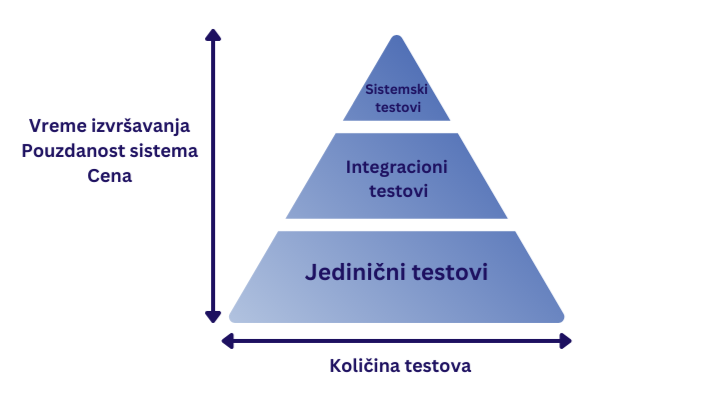
\includegraphics[width=0.8\textwidth]{piramidanova.png}
  \caption{Model piramide testiranja}
\end{figure}

\subsubsection{Testovi jedinica koda}
\par Jedinica je mala logička celina koda: može biti funkcija, klasa, metod klase, modul i slično. Jedinični test proverava samo da li se data jedinica ponaša prema svojoj specifikaciji. Ovi testovi se mogu pisati u potpunoj izolaciji, i ne zavise ni od jedne druge komponente, servisa, ni korisničkog interfejsa. Dakle, izdvajaju se najmanji testabilni delovi aplikacije i proverava se da li rade ono za šta su namenjeni. Ovi testovi su najjednostavniji za pisanje jer se bave malim delom aplikacije, te je kod koji se testira najčešće vrlo jednostavan. 
\par Pri dizajniranju jediničnih testova, nephodno je razmišljati o sledećim ciljevima: 
\begin{enumerate}
\item Dokazati da kod radi ono za šta je namenjen
\item Sprečiti greške --- izmena jednog dela koda može izazvati grešku u nekom drugom delu
\item Utvrditi lokaciju dela koda koji izaziva grešku
\item Napisati najmanju moguću količinu koda za testiranje
\end{enumerate}

\subsubsection{Anatomija jediničnih testova}
\par Kako bi k$\hat{o}$d jediničnog testa bio čitljiv i jednostavan za razumevanje, obrazac četvorofaznog testa (eng. \emph{Four-Phase Test}) predlaže strukturu testa koja podrazumeva ne više od četiri faze \cite{4phase}. Svaki test jedinice koda se može podeliti na četiri jasno odvojive celine:  
\begin{enumerate}
\item Priprema (eng. \emph{Setup}) --- sređivanje podataka koji će se prosleđivati pred samu proveru, često nije neophodna u testiranju čisto funkcionalnih programa.
\item Delovanje (eng. \emph{Exercise}) --- pozivanje koda koji se testira, ključni deo svakog testa.
\item Verifikacija (eng. \emph{Verify}) --- često deo prethodne faze, u ovom delu testovi proveravaju ponašanje koda. 
\item Rušenje (eng. \emph{Teardown}) --- vraćanje podataka na prvobitno stanje, npr. ako se u prvoj fazi koriste neka deljena stanja, kao što je baza podataka. Često implicitno. 
\end{enumerate}

\par Konkretan primer ovako organizovanog testa u programskom jeziku Elm dat je u primeru \ref{lst:4ph}. Definisan je jednostavan test, koji proverava funkciju koja uvećava broj za jedan. U fazi pripreme se broj inicijalizuje na nulu. U fazi delovanja poziva se funkcija testIncrement, zatim se proverava da li je rezultat jednak očekivanom u fazi verifikacije. Faza rušenja u ovom slučaju ne treba da uradi ništa, te jednostavno vraća ().

\begin{lstlisting}[language=elm, caption={Četiri faze jediničnog testa},captionpos=b, label={lst:4ph}]
import Json.Decode as Decode exposing (int)
import Test exposing (..)

-- Setup
setup : Int
setup =
    0

-- Exercise
testIncrement : Int -> Test
testIncrement n =
    let
        result = n + 1
    in
    --Verify
    Expect.equal result 1

-- Teardown
teardown : Int -> ()
teardown _ =
    ()
\end{lstlisting}

\subsubsection{Integracioni testovi}
\label{sec:integration}
\par Jedan od ključnih koraka u razvoju softvera jeste pisanje integracionih testova. Oni utvrđuju da li različite komponente sistema rade zajedno na predviđen način. Pojedinačni moduli i komponente se kombinuju i testiraju kao jedna celina. Cilj integracionog testiranje jeste identifikacija i rešavanje problema koji mogu nastati nakon što se komponente softverskog sistema integrišu i krenu da međusobno komuniciraju. Svaka od njih pojedinačno možda radi kako treba, ali nakon što se to utvrdi jediničnim testovima, potrebno je proveriti da li će njihova interakcija izazvati neželjeno ponašanje. 
\par Integraciono testiranje se može izvoditi na različitim nivoima procesa razvoja --- mogu biti i testovi jedinica koda, sistemski testovi, ili testovi prihvatljivosti\footnote{Vrsta testiranja korisničkog iskustva --- koliko je softver razumljiv i udoban za korišćenje od strane korisnika.} (eng. \textit{Acceptance testing}).
\par U zavisnosti od potreba konkretnog sistema, postoje različiti pristupi integracionom testiranju. Ako su komponente viših nivoa kritične za funkcionalnost sistema, ili od njih zavisi mnogo drugih komponenti, ima smisla prvo testirati njih, pa kasnije postepeno preći na komponente nižih nivoa. Ovakav pristup se naziva testiranje odozgo nadole (eng. \emph{Top-down integration testing}). U suprotnom, ako su komponente nižih slojeva arhitekture kritičnije za celokupan sistem, predlaže se testiranje odozdo nagore (eng. \emph{Bottom-up integration testing}). Hibridno integraciono testiranje (eng. \emph{Hybrid integration testing}) podrazumeva kombinaciju prethodna dva --- započinje sa testovima komponenti najvišeg sloja, zatim se prelazi na testiranje najnižeg sloja, sve dok se postepeno ne stigne do središnjih. Kada je sistem relativno jednostavan i ne postoji veliki broj komponenti, može se primeniti pristup po principu ''velikog praska'' (eng. \emph{Big-bang integration testing}), koji podrazumeva testiranje svih komponenti odjednom, kao jedne celine. 
\par Ako se komponente nalaze u okviru istog sistema, gde postoji kontrola i neko očekivano ponašanje --- integracioni testovi su prilično jednostavni. Međutim, kada su u pitanju spoljašnje komponente i testiranje interakcije sistema sa njima, pisanje integracionih testova postaje malo komplikovanije. Mnoge aplikacije koriste baze podataka, druge servise ili API-je, sa kojima se testovi moraju uskladiti. U testovima se mogu koristiti pravi podaci, ili se umesto njih ubaciti takozvani dubleri (eng. \textit{Test doubles}).
\par Integraciono testiranje je neophodno da bi se obezbedio kvalitetan i pouzdan softver, i zahvaljujući njemu rano se uočavaju različiti problemi do kojih može doći i time značajno redukuje vreme i cena celokupnog razvoja. 

\section{Testiranje funkcionalnih programa}

\par Čiste funkcije samo uzimaju argumente i proizvode izlaz, ne prave nikakve izmene niti imaju skrivene izlaze. Koriste imutabilne vrednosti, i time olakšavaju pronalaženje određenih problema u programima. Testiranje i debagovanje ovako napisanih programa postaje mnogo jednostavnije. Najvažnija stvar kod testiranja u funkcionalnoj paradigmi jeste pisanje čistih funkcija i njihovo testiranje u izolaciji, kako bi se obezbedila ispravnost i robustnost. Takođe je važno da se ne testira samo uspešan scenario, već i granični slučajevi, kao i slučajevi greške.

\subsection{Testiranje čistih funkcija}

\par Najjednostavniji kod za testiranje jeste čista funkcija. Ako postoji bilo kakva izmena u podacima, takva funkcija nije čista. Pri testiranju čiste funkcije, s obzirom da ne postoje propratni efekti, test može da se fokusira samo na dve stvari: ulazne podatke i na sam izlaz funkcije. 
\par Kada je u pitanju čista funkcija, jedina priprema koja je potrebna jesu podaci koji će se proslediti kao parametri. Drugi korak jeste poziv funkcije, sa prosleđenim argumentima. Faza verfikacije su samo provere nad rezultatom, i samo nad rezultatom. Testovi su veoma jednostavni jer ne moraju da brinu o bočnim efektima i njihovim neželjenim posledicama, i uvek će dobijati  isti odgovor od testiranog koda, ma koliko puta bili pokrenuti. 
\par Aplikacije se u većini slučajeva neće sastojati od isključivo čistih funkcija, i u vezi sa tim postoje dve strategije \cite{testingelixir}. Prva je izdvojiti logiku u čiste funkcije, a druga dizajnirati funkcije tako da koriste neku od metoda ubrizgavanja zavisnosti (eng. \textit{Dependency injection}) \footnote{Ubrizgavanje zavisnosti je obrazac u kom objekat ili funkcija prihvata druge objekte ili funkcije od kojih zavisi. Jedan od oblika inverzije kontrole, za cilj ima da razdvoji konstrukciju i upotrebu objekata i time smanjuje spregnutost programa.}, što omogućava izolaciju koda.

\subsubsection{Refaktorisanje ka čistim funkcijama} 
% TODODO modul - funkcija, plus ovo je konkretno za elixir koji nije cist, plus slike treba dati konkretan primerrr!
Ako je neki deo koda komplikovan za testiranje, najlakši način da se pojednostavi jeste refaktorisati ga u čistu funkciju, ukoliko je to moguće. Deo koda koji zavisi od nekog drugog dela iz spoljašnjosti će u većini slučajeva pozivati tu spoljašnju zavisnost i onda manipulisati rezultatom pre nego što vrati svoj rezultat. Što više takve manipulacije ima, to je taj deo koda bolji kandidat za premeštanje logike unutar čiste funkcije. Na slici \ref{fig:dep} su date vizuelne reprezentacije kako ovaj proces izgleda pre i posle izmeštanja koda u čistu funkciju. 
Na početku, funkcija može biti komplikovana za testiranje. Svaki test, za svaki mogući način ponašanja bi nekako morao da garantuje da druga funkcija (ona od koje zavisi prva) vraća neki očekivani odgovor. Ideja je da se deo logike (na slici označen sa ``manipulacija podataka ``) izvuče van --- u novu, čistu funkciju. Tako postaje zasebna komponenta, koja se može odvojeno lako testirati. Kada je taj deo logike dobro istestiran, može se smatrati sigurnim da se ponovo pozove u originalnoj funkciji. Zna se da će taj čisti kod uvek vraćati isti rezultat, i može se značajno redukovati broj testova neophodnih za testiranje originalne funkcije. U primeru koda... TODO primer

\begin{figure}[!ht]
  \centering
  \label{fig:dep}
  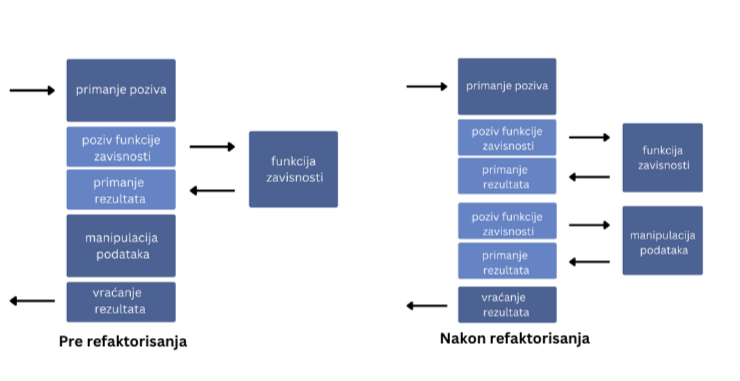
\includegraphics[width=0.9\textwidth]{dep.png}
  \caption{Izmeštanje koda u čistu funkciju}
\end{figure}

\par  U nekim slučajevima, nije lako odrediti šta se može izdvojiti u zasebnu funkciju. Tada postoji druga opcija za kreiranje kontrolisanog okruženja: napraviti zamenu za funkciju zavisnosti, i time izolovati kod. 

\subsection{Izolovanje koda} 
\par Ubrizgavanjem zavisnosti i kreiranjem dublera moguće je eliminisati spoljašnje promenljive, i time kontrolisati situaciju u kojoj k${o}$d koji se testira mora da se nađe. Tako se omogućava očekivanje nekog konkretnog rezultata. 
\par Zavisnost je bilo koji kod na koji se originalni kod oslanja. Korišćenjem DI (skraćenica za Dependency Injection) u testovima se kreiraju zamene zavisnosti koje se ponašaju na predvidljiv način, pa testovi mogu da se fokusiraju na logiku unutar koda koji se testira. U jediničnim testovima, najčešće se ubrizgava zavisnost tako što se prosledi kao parametar. Taj parametar može biti funkcija ili modul. Ubrizgavanje zavisnosti kroz API\footnote{skraćenica za aplikacioni veb interfejs (eng. \textit{Web Appilicatoin
Programming Interface} )} obezbeđuje čist kod i jednostavne i kontrolisane jedinične testove. Sa druge strane, integracioni testovi zahtevaju drugačije metode ubrizgavanja zavisnosti. TODO nastavak...


%TODO
\par TODO ovde ide jos....
% ------------------------------------------------------------------------------

\chapter{Portal MSNR}
\label{chp:msnr}

%TODO 
\par Ovde ide opis aplikacije koja se testira.... \cite{msnr-portal} \cite{rad}

\par Testiranje različitih slojeva aplikacije MSNR portal će u nastavku rada biti sprovedeno u narednim koracima. Za početak će se testirati individualne funkcije i upravljači koji barataju zahtevima i odgovorima u okviru koda za serverski deo aplikacije napisanog u Elixir programskom jeziku pomoću razvojnog okvira Phoenix. Nakon toga, potrebno je testirati integraciju aplikacionog interfejsa sa bazom podataka --- integracioni testovi koji simuliraju zahteve API-ju i verifikuju odgovore od baze. TODO jos ovde o tome .... 

\chapter{Testiranje serverskog dela aplikacije}
\label{chp:elixir}

Serverski deo aplikacije MSNR portal napisan je na programskom jeziku Elixir. Elixir je vrlo specifičan jezik, sa konceptima koji mogu biti komplikovani za testiranje. Nije čist funkcionalni jezik, i dinamički je tipiziran. Konkurentost i imutabilnost kao osobine su prisutne i u drugim jezicima, ali na primer rezilijentnost ili OTP (eng. {Open Telecom Platform}) razvojni okvir su vrlo jedinstveni za Elixir (i Erlang). Elixir se prevodi na isti bajtkod kao i Erlang, i pokreće se na Erlang virtuelnoj mašini, poznatoj pod nazivom BEAM.. . jos o elixiru ... Referenca na zvaničnu stranicu \cite{elix} TODO %TODO REF. 
U većini slučajeva, kod napisan u Elixir-u zavisi od nekoliko Erlang biblioteka. Međutim, kada je testiranje koda u pitanju, alati i biblioteke koji se koriste su jedinstveni za svaki od ova dva jezika. Ovde će se govoriti o testiranju isključivo Elixir koda. 

Zajedno sa ovim jezikom dolazi njegov razvojni okvir za testiranje, ExUnit \cite{exunit}. U ovom poglavlju biće predstavljeni različiti koncepti testiranja u programskom jeziku Elixir, kroz pisanje testova za serverski deo aplikacije MSNR portal. Na primeru ove aplikacije, objašnjeni su načini pisanja testova za funkcionalni kod. U narednim sekcijama, prikazano je testiranje važnih osobina Elixir programskog jezika, kao što su tipovi podataka, OTP razvojni okvir, Ecto \cite{ecto}, Phoenix razvojno okruženje\cite{phoenix}.

\section{Testiranje jedinica koda}

\textit{ExUnit} je Elixir-ov ugrađeni razvojni okvir koji ima sve što je neophodno za iscrpno testiranje koda i biće osnova za sve testove kroz ovo poglavlje. S obzirom na to da je Elixir funkcionalni jezik, može se diskutovati o tome šta se smatra "jedinicom". Uobičajeno je da se jedinični testovi fokusiraju na pojedinačnu funkciju i njenu logiku, kako bi se opseg testa održavao što užim, radi bržeg pronalaženja grešaka. Međutim, nekada ima smisla da se u opseg testa uključi više modula ili procesa, i time se proširi definicija jedinice koda. Znati kada treba proširiti taj opseg može mnogo uticati na smanjivanje kompleksnosti i održavanje samih testova. 

\par Pisanje testova u programskom jeziku Elixir je moguće bez potrebe za drugim bibliotekama, jer razvojni okvir ExUnit je razvijan zajedno sa samim jezikom od početka. U ovom delu, biće prikazani jednostavni jedinični testovi, koji će prikazati neke osnovne koncepte koje nudi ExUnit. 

\par Svita testova (eng. \emph{Test suite}) je kolekcija testova slučajeva upotrebe, koji imaju isti posao, ali različite scenarije. Ona može služiti kao dokumentacija, sa opisima o očekivanom ponašanju koda, tako da treba voditi računa da bude dobro organizovana. ExUnit dolazi sa veoma korisnim funkcijima i makroima koji omogućavaju tu organizaciju u jednu čitljivu i održivu  datoteku. Alat \emph{describe } omogućava davanje opisa grupe testova, kao i dodeljivanja zajedničke pripreme podataka za celu grupu. Preporuka je za početak grupisati testove po funkciji, kao što je prikazano u primeru koda \ref{lst:desc}, ali odluka o načinu grupisanja je na pojedincu. Svrha je čitljivost i lakše razumevanje. 

\begin{lstlisting}[language=elixir, caption={Opisivanje testova unutar jedne grupe},captionpos=b, label={lst:desc}]
defmodule MyApp.ModuleTest do 
   use ExUnit.Case 
   
   describe ''thing_to_do/1'' do
   	test ''it returns :ok, calls the function if the key is correct''
   	test ''it does not call the function if the key is wrong''
   end
end
\end{lstlisting}

\par Testovi u Elixir projektima se uglavnom čuvaju u direktorijumu projekta \textit{'/test'}, i organizuju se u module i test slučajeve. U prethodnom primeru koda, modul pod nazivom ModuleTest se sastoji od dva test slučaja. 

\subsection{Pisanje ExUnit testova}
\par Za svaku funkciju ili upravljač potrebno je napisati test slučajeve. Jedan test slučaj se sastoji iz funkcije testa koja poziva funkciju ili upravljač i proverava očekivani rezultat.  



\par ovde jos ... , primeri , ... 


\section{Integraciono testiranje}
\par Nakon dobro istestiranih pojedinačnih funkcija i modula, potrebno je proveriti da li komponente funkcionišu ispravno kao celina. U ovom poglavlju biće prikazani testovi koji proveravaju da li različiti delovi sistema koji komuniciraju međusobno, kao i sa nekim eksternim sistemima, rade to na ispravan način.

\subsection{Test dubleri}

\par 

\subsection{Neki podnaslov}
U aplikaciji MSNR portal --- TODO konkretni primeri ... 

\chapter{Testiranje klijentskog dela aplikacije}
\label{chp:elm}

\chapter{Integracija klijentske i serverske strane}
\label{chp:elmelixir}

\chapter{Testiranje celokupnog sistema --- End to End}
\label{chp:e2e}

% ------------------------------------------------------------------------------
\chapter{Zaključak}
% ------------------------------------------------------------------------------

% ------------------------------------------------------------------------------
% Literatura
% ------------------------------------------------------------------------------
\literatura

% ==============================================================================
% Završni deo teze i prilozi
\backmatter
% ==============================================================================

% ------------------------------------------------------------------------------
% Biografija kandidata
%\begin{biografija}

%\end{biografija}
% ------------------------------------------------------------------------------

\end{document}
